\documentclass[tikz,border=10pt]{standalone}
\begin{document}
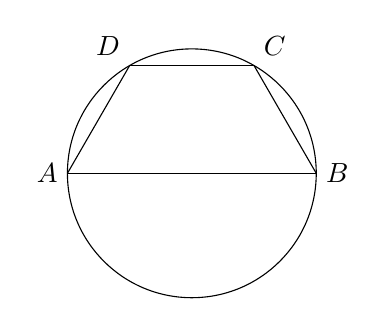
\begin{tikzpicture}
  \coordinate (A) at (-1.58,0);
  \coordinate (B) at (1.58,0);
  \coordinate (C) at (0.79,1.368);
  \coordinate (D) at (-0.79,1.368);
  \coordinate (O) at (0,0);

  \draw (O) circle (1.58);
  \draw (A) -- (B);
  \draw (B) -- (C);
  \draw (C) -- (D);
  \draw (D) -- (A);

  \node[above left] at (D) {$D$};
  \node[above right] at (C) {$C$};
  \node[left] at (A) {$A$};
  \node[right] at (B) {$B$};
\end{tikzpicture}
\end{document}
